
\documentclass[12pt]{article} % article class, 12pt font

% load any packages you need for more custom stuff
\usepackage[margin=1in]{geometry} % set 1-inch margins
\usepackage{setspace}\doublespacing % set double spacing
\usepackage[superscript]{cite} % superscript numeric in-line citations
\usepackage{indentfirst} % indent the first paragraph of each section
\usepackage{graphicx} % enable displaying png format graphs
\usepackage{csvsimple} % enable importing tabular data
\usepackage{booktabs} % enable formulating tables


% set title stuff
\title{The Spread of Disease}
\newcommand{\authors}{Eli Sylvia-Lourde}
\author{Math 114 Mathematical Modeling\\St. Mary's College}
\date{February 22, 2019}

% start the actual document
\begin{document}

% create title stuff
\hfill\authors % write the authors right-aligned
%\vspace{-0.5in} % reduce space before title
{\let\newpage\relax\maketitle} % print title

% begin the main text
\section*{Problem Statement}
An	isolated	town	has	a	population	of	100,000	residents.	Last	week	there	were	18 new	cases	of
people	infected	by	a	mild	disease	that	lasts three	weeks and	leaves	the	person	immune	from
further	disease.	Direct	contact	with	an	infected person	leads	to	an	infection	of	a	previously
uninfected	person.	This	week	there	are	40 new	cases.	It	is	estimated	that	30\% of	the	existing
population	is	immune	because	of	previous	exposure.

\begin{enumerate}
\item
Make	a	list	of	assumptions	that	you	need	to	make	in	order	to	develop	a	dynamical
system	model	using	difference	equations.
\item
Develop	a	model	that	describes	how	the	number	of	new	cases	each	week	develops.
\item
What	is	the	eventual number	of	people	who	will	become	infected?
\item
Vary	the	assumptions	you	make	in	this	model	to	develop	a	feel	for	how	sensitive	the
model	is	to	your	assumptions.
\end{enumerate}

\section*{List of Assumptions}
\begin{itemize}
\item
Every person in the population is equally exposed to any peoples that are infected.
\item
Every person that is exposed to an individual that is infected has the same chance of becoming infected themselves.
\item
That the first week the infection is introduced into the population, 18
people develop cases of the sickness.
\item
That the second week the infection is introduced into the population, 40
people develop cases of the sickness.
\item
People recover on their third week on getting the disease, not after their third week of getting the disease.
\item
That the 30\% of people that are immune in week 2 are immune via genetic trait.
\end{enumerate}

\section*{The Model}
Based upon an equation given by the book, (Section 1.2|Example 3|p.13) we can assume that the spread of
disease can be modeled with the following equation: \linebreak $\Delta i_{n} = i_{n+1} - i_{n} = ki_{n}(N-i_{n})$
, where $i_{n}$ is the number of people that developed the disease on week $n$, $k$ is a constant, and $N$ is the total
population. In this equation, $i_{n}(N-i_{n})$ represents the number of times an infected person will come into contact with someone who can become sick. $k$ is the probability that someone will become sick if they encounter someone that is infected. Unlike the equation in the book, the people in the problem statement will get better after 3 weeks of having the disease. Also, we don't only care about the spread of disease, but rather the total number of people that are infected. This is reflected in the following equation:
 $ \displaystyle i_{n+1} = i_{n} + ki_{n}(N-i_{n}-s_{n}) - \Delta i_{n-2}$.
This reads as the following: the number of people that have the disease in week n+1 is equal to the number of people that have the disease in week n plus the number of people that contracted the disease in week n+1, minus the number of people that have become immune to the disease. The number of people that have contracted the disease is calculated by multiplying the constant k, the number of people that had the disease on week n, and the number of people that are succeptible to the disease. The number of people succeptible to the disease is found by subtracting the number of sick people on week n and the number of immune people on week n. The constant, k is found by calculating the number of infected individuals for week one. Given that week zero had 18 infected, and week one had 58 infected, we are able to solve for succeptible population, which eventually allows us to find out k-value (k=0.00057157).

\section*{People Who Become Infected}


% 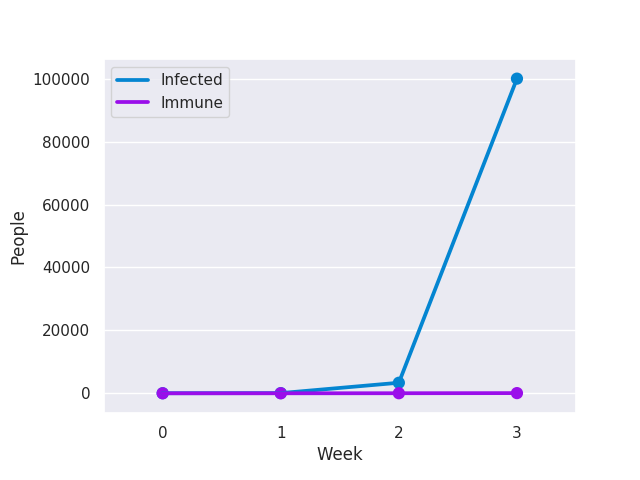
\includegraphics{Actual_Spread.png}
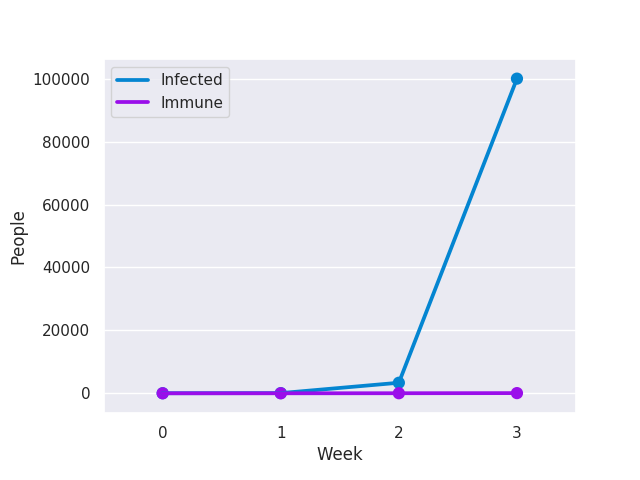
\includegraphics{Actual_Spread.png}

As shown by the figure above, the disease infects everyone by week three. If we decrease our k-value by a factor of fifteen, everyone is immune to the disease by week 8.

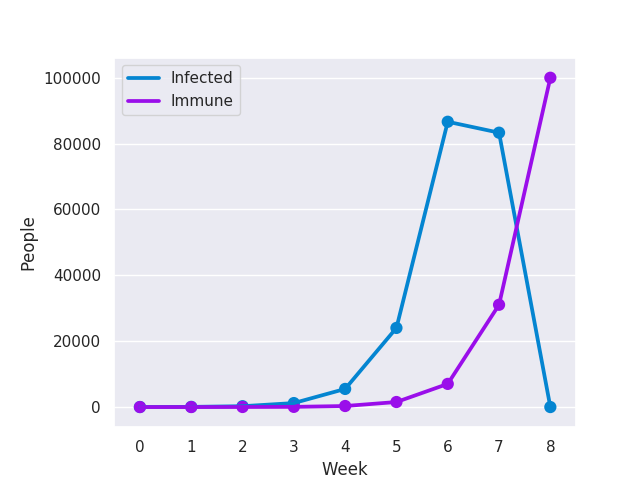
\includegraphics{humans_win.png}

If we continue to decrease the k-value, the infection spreads slower, which leads to it doing less and less damage to the given population. It would be interesting to make the model more complicated by having a certain percent of those that are infected die, or a certain percent of those that are immune loosing their immunity.

%
% As shown by the figure above, the number of people that have the disease peaks at 114, with the number of immune people finishing at 343. Given that k affects how quickly our disease spreads, we might wish to check the accuracy of our constant. We can do this by looking at the slope of the above figure for weeks [0,2]. Given that the slope between these two weeks looks fairly linear, we assume that we have calculated our k correctly (k=0.00057157). In order to test how sensitive our model is to different k-values, the following two figures are the result of our model being ran for k = 0.05 and k=0.75. If k was less than 1, the infection would infect the entire population.

% 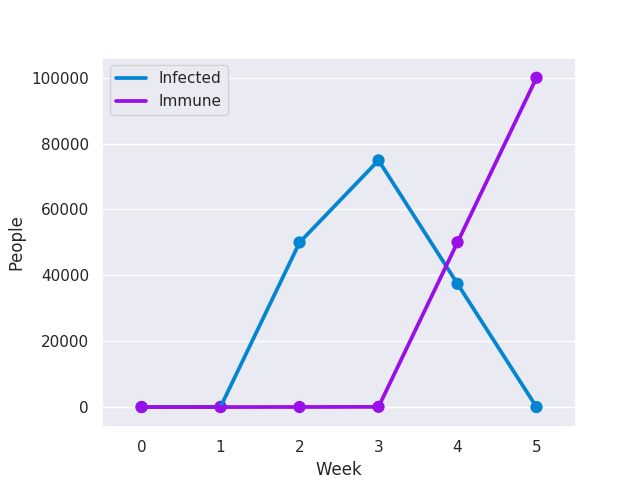
\includegraphics{K_05.png}
% 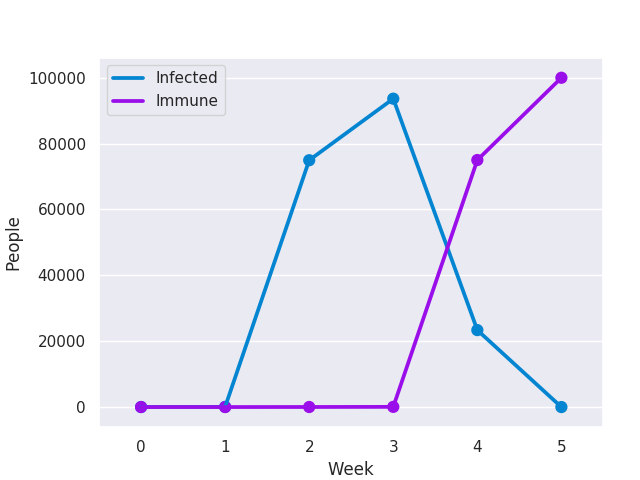
\includegraphics{K_75.png}


% \section*{Conclusions}
% The conclusion should address the solutions to the problem in a straight forward fashion. The results should be in terms that the one posing the question can understand. Frequently questions requiring a model are stated in non-technical terms, and so the answer should stated in a way that the person posing the question can understand.
%
\end{document} % this ends your document
